\chapter{Implementation}

\section{Issues Encountered During Implementation}

\subsection{Creating tables using bootstrap}

Initially it was decided to create the SQL tables during visualisation using the Bootstrap 5 Grid system. Using a series of rows and column in a flexbox it can layout and align the content dynamically. This seemed like a good tool for creating tables because it allowed for creation of custom layouts for tables and it would give more freedom for styling and highlighting since it is not a restrictive structure of a HTML table element. This was the reason that HTML tables were not used for this because the table cells will be empty since the SQL parsing will not be done for "INSERT" statements so no entries will be added to the tables.

Later on in the implementation of this tables when the parsing was sophisticated enough to parse large tables, the problem emerged of Bootstrap shifting the layout of the tables and squashing it's columns together to look like rows on smaller screen or if the window was resized. The grid system is useful when building layouts for mobile-first designs and the changing the layout when the screen size is smaller is useful, but not for this project since learners are not going to be writing their sql databases on a mobile device. 

\begin{figure}[h!]
	\centering
	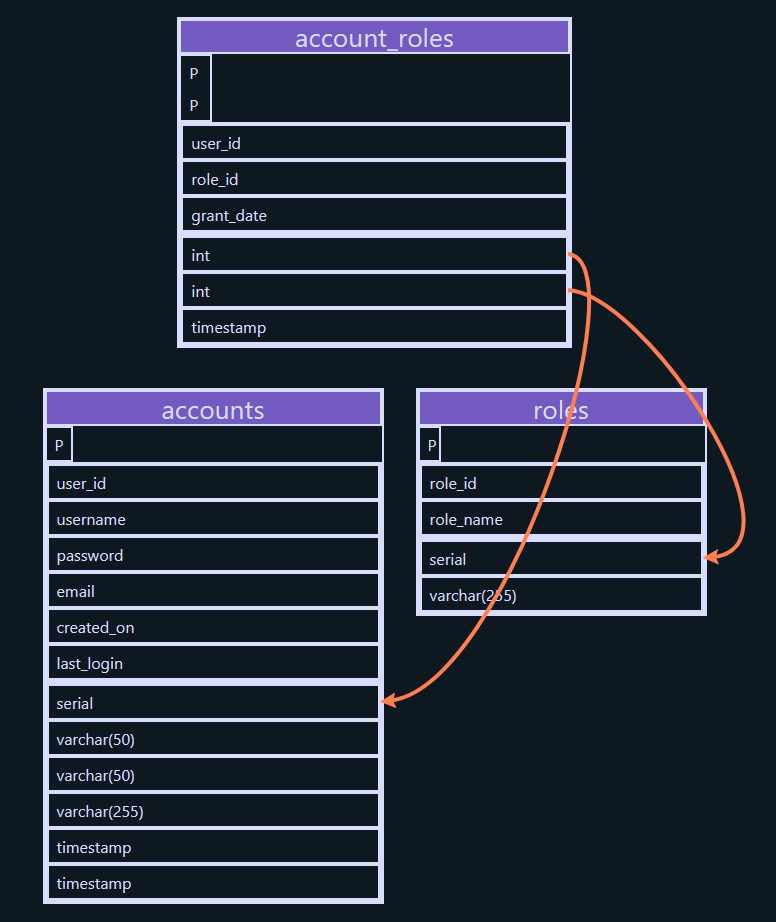
\includegraphics[scale=0.5]{postSquash}
	\caption{Visualisation of tables showing the column being compressed to look like rows in a single column due to the flexbox responsive resizing.}
	\label{fig:squash}
\end{figure}

This problem was solved by going back to using HTML table elements and dynamically creating tables from the table objects. This solution was slightly harder to implement however the and layout was much better since Bootstrap did not resize the table element. This was because the entire table is viewed as an element which prevents it from being changed when the window is resized, compared to the previous implementation which had a single column be an element which was resized. Bootstrap provides styling classes for tables which made the styling easy to change as it was before using the previous tables.

\begin{figure}[h!]
	\centering
	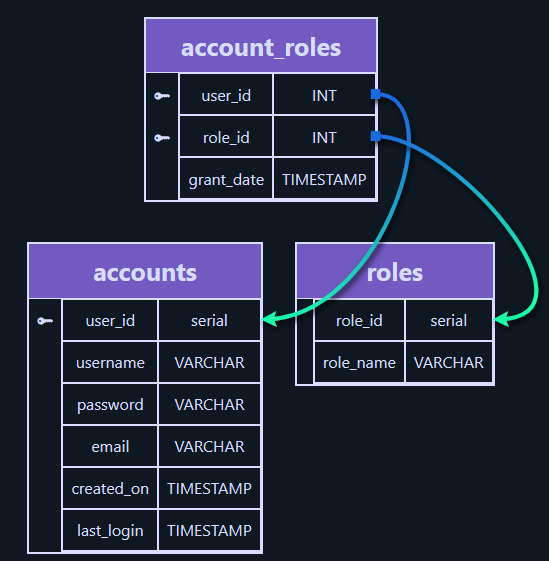
\includegraphics[scale=0.7]{newPostSquash}
	\caption{Visualisation of tables after a structure using HTML table elements was adopted, showing no signs of distortion after changing the size of the window.}
	\label{fig:afterSquash}
\end{figure}

\subsection{Early stages of parsing}

Early stages of parsing used simple checking of strings and struggled separating spaces properly, as well as punctuation and created complex regular expressions that were hard to read and were prone to break. Used the tokenising library that made it easier to create some data structure that was easy to work with and made the parsing a lot easier. Parsing was a lot more complex than initially thought. Lot's of edge cases for SQL and an immense complexity in the number of possible statements and combination of statements. Lot of work went into implementing parsing for just a few statements however, this just took a longer time to write than expected but it was done.

\subsection{Drawing arrows library}

Drawing lines between two HTML elements was something that had to be done to represent foreign key relationships between tables. One possible way to do was to use a HTML canvas and draw lines using the elements positions. However this was difficult to style correctly to match the design and would require more work to create a function to do what is required. Instead, a library leader-line \cite{leader-line} was used to draw an arrow between two elements. The styling of this arrows was much easier to do and it also included some implementation for animations which made the design look much better.

\subsection{Drawing Tables on the webpage}

Drawing the tables in a way that was easy to understand was difficult because the order or layout the tables are displayed in plays a key role in how easy a database can be understood. It was first implemented to display the tables in the order in which the tables appeared in the SQL text file since it seemed logical to do so because the learners will expect the tables to be displayed in this order. However once foreign key arrows were implemented then the tables had foreign key constraint arrows across them because the tables that were joined together were not together in the sql text file. This was quite confusing to try to understand and a decision was made to display them in a more organised structure. 

\begin{figure}[h!]
	\centering
	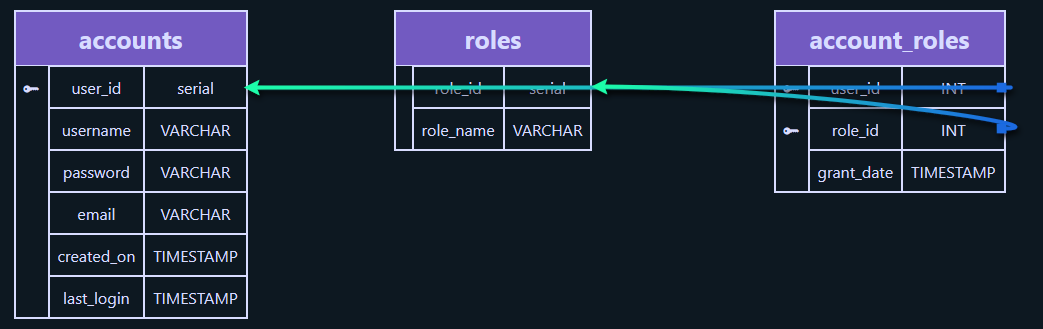
\includegraphics[width=\textwidth]{overlap}
	\caption{Visualisation of tables in the order of creation with drawing of arrows depicting overlap between the tables and arrows prevent text in columns to be readable.}
	\label{fig:overlap}
\end{figure}

\subsection{Representation of Missing Keys}

%talk about instant feedback that a primary key is missing, integral part of the design that should be fixed. Need to be represented in the table view since primary keys are shown in the table. Before it was just red outline in key column so hard for user to figure out what the problem is. After the entire table is red and there is a tooltip to inform the user of what is wrong. 

\subsection{Implementing Highlighting of Text in a HTML TextArea}

The HTML Textarea is what is used in the website form to enter the SQL text by the user, to be user-friendly, if the entered SQL has some syntax errors it should highlight roughly where the error is. This is important because an SQL learner will not be able to easily spot where their error is in the SQL, since they are not familiar with the syntax. 

\begin{figure}[h!]
	\centering
	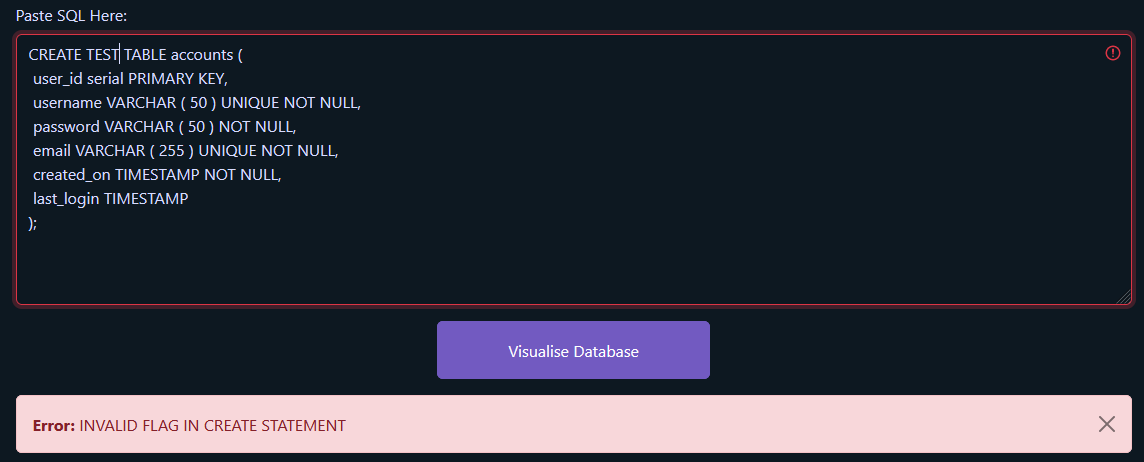
\includegraphics[width=\textwidth]{textArea}
	\caption{Initial implementation of the textArea validation and syntax error alert.}
	\label{fig:textArea}
\end{figure}

The HTML Textarea does not natively have the functionality to highlight text inside of it, any mark up to the text would appear as plain text. A possible solution to this problem is to implement a rich text editor in the webpage and replace the Textarea with it, rich text areas can provide implementation to highlight and mark up text much better and easier than the Textarea. However building a rich text editor is not the easiest to do since even basic functionality is difficult to implement \cite{highlightText}.

However since adding a already functioning text editor to the webpage would require styling it and cutting down all of the features down only to the highlighting, it was decided to create a work around for the Textarea. This was done by creating a "fake" textarea under the current one that only looked like a textarea and since it was overlayed over the textarea, it was not perceivable by the user. The goal of this textArea is to only highlight the text and since it is a div that looks like a textArea this can be done by creating span elements of the words that have to be highlighted that had some styling. This proved to be quite easy to implement and provides the solution to the problem.

\begin{figure}[h!]
	\centering
	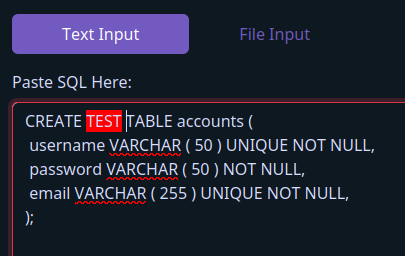
\includegraphics[scale = 1]{highlightedTextArea}
	\caption{Later implementation of the highlighting of the origin of the syntax error in the input textarea.}
	\label{fig:highlightedTextArea}
\end{figure}

\newpage

\section{Review of Requirements}

The initial requirements are all mostly met apart from the functionality that is outside the scope of this project that is mentioned previously in the report. 

\begin{center}
	\captionof{table}{\label{fig:reviewOfImplementation}Table reviewing the initial table of requirements}
	\setlength\extrarowheight{2pt}
	\begin{tabularx}{\textwidth}{|X|X|X|}
		\hline
		\textbf{Functional Requirement Number} & \textbf{Functional Requirement Name} & \textbf{Review of Requirement} \\
		\hline
		FR-1 &  Enter SQL into website form & The user can enter their SQL in either text form in the textarea or in file form by uploading their file into the filepicker. The website processes the correct data that the user provides. \\
		\hline
		FR-2 & Validate entered SQL & Once the data has been entered the SQL is validated and feedback is given to the user through the styling of the form and the alerts whether the SQL is correct or has syntax errors. \\
		\hline
		FR-3 & Visualise entered database & The entered database is visualised by creating tables and the links between them.\\
		\hline
		FR-4 & View highlighted syntax after visualising & Once the database has been visualised, the "syntax view" tab can be selected to find the highlighted and indented SQL that had been entered before. \\
		\hline
		FR-5 & The user can filter through data types of columns in syntax view & At the syntax view tab there are filters that can be checked to highlight the data types to a green colour to separate them from the rest. \\
		\hline
		FR-6 & The user can view the flaws of the database & Once the database has been visualised, the "Problem View" tab can be selected with a list of flaws that the database might have, if there are no flaws detected then the user is prompted with a message. \\
		\hline
	\end{tabularx}
\end{center}